El cable es un elemento flexible que, sujeto a cargas externas, adquiere una forma concreta llamada funicular, que depende de la magnitud y la posición de las mismas, la forma que adopta el cable al estar sujeto en sus extremos y expuesto a la acción de su propio peso es justamente la catenaria.
\begin{figure}[h]            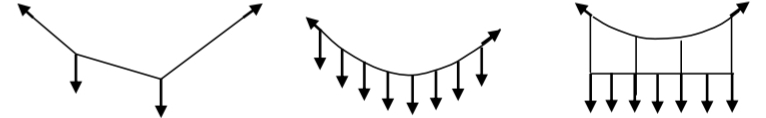
\includegraphics[width=10cm]{Imagenes/FormasCat.jpg}
    \caption{Formas que adoptan los cables al estar someditos a diferentes cargas.}
    \centering
\end{figure}

\framebreak
Las estructuras atirantadas se han utilizado extensamente a lo largo de la historia, hay muchos ejemplos de puentes colgantes con materiales tipo bambú, cañas o cuerdas. Más actualmente se han construido un gran número de edificios con estructuras de cables, siendo el acero galvanizado y el acero inoxidables los materiales más usados actualmente.
      \begin{figure}[h]
        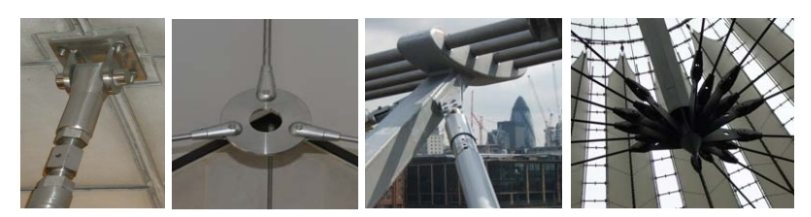
\includegraphics[width=10cm]{Imagenes/UnionesCat.jpg}
        \caption{Uniones de Cables.}
                \centering
            \end{figure}

\framebreak
Entre las estructuras que utilizan a los cables, o se sirven de la forma de la catenaria, podemos encontrar los siguientes grupos
\begin{itemize}
    \item Estructuras soportadas por cables
    \item Estructuras superficiales formadas por cables.
    \item Estructuras con arcos catenarios como columnas de apoyo.
\end{itemize}
\framebreak
\textbf{Estructuras  soportadas por cables:}
\\Se caracterizan porque los cables trabajan individualmente, como elementos suspendidos o como columnas a tracción, para soportar elementos estructurales como vigas, superficies o edificios.
    \begin{figure}[h]
       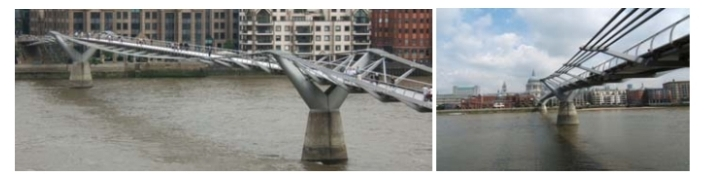
\includegraphics[width=10cm]{Imagenes/Mill Lon.jpg}
            \centering
            \caption{Millenium Bridge, Londres.}
    \end{figure}

\framebreak
Un ejemplo de edificio soportado por cables es el banco de la reserva federal de Mineapolis, de Gunnar Birkerts (1973) en el que de dos cables anclados a dos núcleos de hormigón separados 100 m cuelgan 11 plantas.
    \begin{figure}[h]
       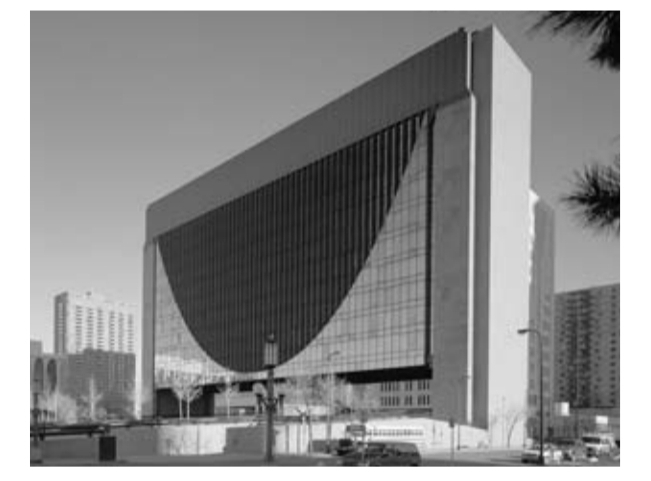
\includegraphics[width=5cm]{Imagenes/BancoR.jpg}
                \centering
                \caption{Banco de la reserva federal, Mineapolis}
    \end{figure}

\framebreak
\textbf{Estructuras  superficiales formadas por cables:}
\\Se caracterizan porque los cables trabajan conjuntamente formando estructuras superficiales o incluso bidimensionales.
\\Se utilizan fundamentalmente para cubiertas y, en ellas, los cables se disponen paralelamente o de forma radial, llegando a cubrir luces de entre 45 m y 135 m\footcite{Lui15}
    \begin{figure}[h]
       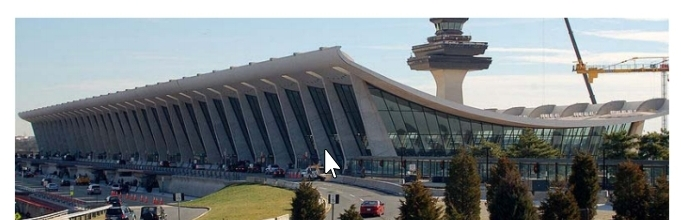
\includegraphics[width=10cm]{Imagenes/Aeroupuerto.jpg}
                \centering
                \caption{Terminal del aeropuerto de Dulles}
    \end{figure}

\framebreak
\textbf{Estructuras  con arcos catenarios:}
\\Antoni Gaudí, arquitecto español de mediados del s. XIX, trabajó un sistema estructural basado en la mecánica y la geometría de las curvas funiculares, a partir de la observación de formas orgánicas en la naturaleza.
    \begin{figure}[h]
       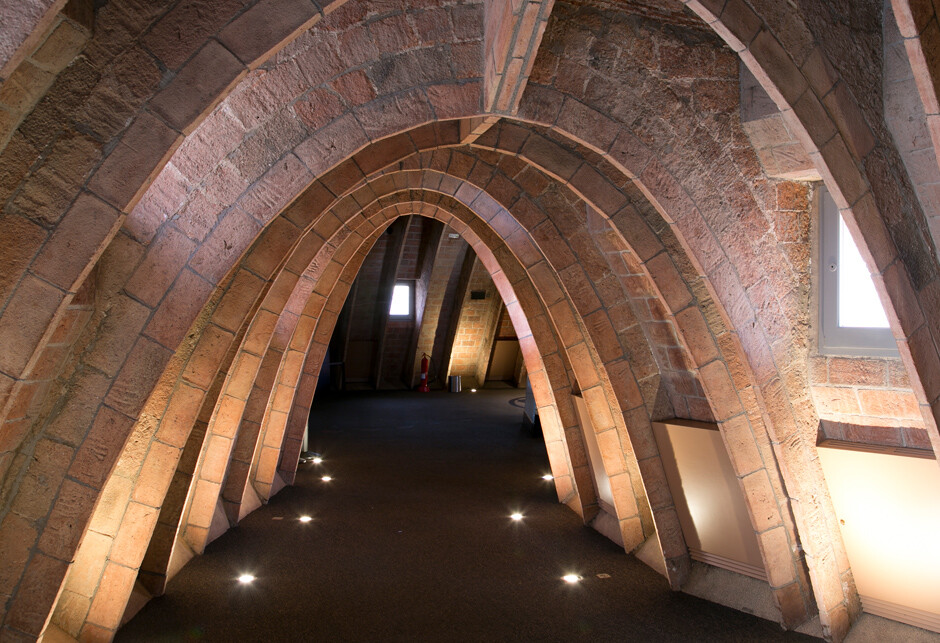
\includegraphics[width=6cm]{Imagenes/ArcosCate.jpg}
       \caption{Arcos catenarios de Gaudi}
                \centering
    \end{figure}

